
\documentclass[12pt, a4paper]{article}

\usepackage[utf8]{inputenc}
\usepackage[T1]{fontenc}
\usepackage[russian]{babel}
\usepackage[oglav,spisok,boldsect,eqwhole,figwhole,hyperref,hyperprint,remarks,greekit]{./style/fn2kursstyle}
\graphicspath{{./style/}{./figures/}}

\usepackage{multirow}
\usepackage{supertabular}
\usepackage{multicol}
% Параметры титульного листа
\title{Кручение стержня\\ прямоугольного сечения}
\author{В.\,Г.~Пиневич}
\supervisor{А.\,В.~Котович}
\group{ФН2-51Б}
\date{2023}

% Переопределение команды \vec, чтобы векторы печатались полужирным курсивом
\renewcommand{\vec}[1]{\text{\mathversion{bold}${#1}$}}%{\bi{#1}}
\newcommand\thh[1]{\text{\mathversion{bold}${#1}$}}
%Переопределение команды нумерации перечней: точки заменяются на скобки
\renewcommand{\labelenumi}{\theenumi)}
\begin{document}

\maketitle

\tableofcontents



\newpage

\section-{Введение}
Проблема решения задачи о скручивании балки возникает во многих задачах, в частности в строительной механике. <Что-то написать здесь>. Данная работа посвящена изучению двух численных методов решения таких задач, оценке их точности.

\section{Постановка задачи}
\subsection{Кручение}
Кручением называется такой вид нагружения стержня, при котором
из всех шести внутренних силовых факторов в его поперечных сечениях не равен нулю только крутящий момент~$M_{\text{кр}}$.

Рассмотрим стержень прямоугольного сечения. 
Такой стержень при
закручивании подвержен депланациям («выходят из плоскости»). Другими словами депланация означает, что точки сечения перемещаются вдоль оси стержня
в различных направлениях.
\begin{figure}[!h]
	\centering
	\includegraphics[width=0.35\textwidth]{sterzhenСruchenie}%
	\caption{Кручение стержня прямоугольного сечения}
	\vspace*{-2mm}
	\label{pic1}
\end{figure}

Будем решать задачу о его кручении двумя способами: энергетическим методом (в виде ряда по ортогональной системе функций) и методом Ритца (в виде ряда по степенным функциям).

Совместим ось $z$ с осью кручения, оси $x$ и $y$ расположим произвольно в плоскости поперечного сечения. Задача кручения сходится к поиску функции $\psi$~(\ref{funCruc})~\cite{Temochenko75}. Эта функция должна быть постоянна вдоль границы поперечного сечения, константу можно выбирать произвольно. Мы будем принимать ее равной нулю.
\begin{equation}
	\label{funCruc}
	\Delta \psi = \frac{\partial^2 \psi }{\partial x^2} +
	\frac{\partial^2 \psi }{\partial y^2} = -2G \theta, 
\end{equation}
\noindent где $G$ --- модуль сдвига, $\theta$ --- угол закручивания на единицу времени.


\subsection{Положительные и положительно определенные операторы}
Рассмотрим некоторый симметричный оператор $A$ гильбертова пространства.
\begin{itemize}
	\item [$\bullet$]
Оператор $A$ называется положительным,
если для любого элемента $u$ из области определения оператора
выполняется неравенство
\[
(Au, u) \geqslant 0,
\]
причем знак равенства имеет место только тогда, когда $u = 0$.
\item [$\bullet$]
Оператор $A$ называется положительно определенным, если существует такая положительная постоянная $\gamma^2$, что для любого элемента $u$ из области определения оператора $A$ справедливо неравенство
\[\label{positive_definite_operator_1}
	(Au, u) \geqslant \gamma^2 \|u\|^2
\]
\end{itemize}

Физический смысл понятия положительно определенного
операторов заключается в том, что невозможно сообщить
системе смещение, не затратив на это некоторой энергии~\cite{MICHLIN_SMOLICKY}. Если же оператор положительный, но не положительно
определенный, то, системе можно придать сколь угодно большое смещение, затратив на это сколь угодно малую энергию

\section{Энергетический метод}
Рассмотрим положительно определенный оператор $A$ в гильбертовом пространстве $H$. Требуется решить уравнение 
\begin{equation}
	\label{craev_task}
	Au = f, f \in H. 
\end{equation}

Пусть $A$ --- положительный оператор в гильбетровом протестантстве. Тогда энергетическим произведение назовем 
\[
	[u, v] = (Au, v),
\]
\noindent где $u$ и $v$ элементы из области определения $D$ оператора $A$. 

Множество $D(A)$ является гильбертовом пространством, навезем его энергетическим пространством $H_A$. Оно также является сепарабельным.

Тогда мы можем свести решение краевой задачи к задаче о поиске минимума функционала.

Если $A$ --- положительный оператор, уравнение~(\ref{craev_task}) можно свести к поиску минимума функционала
\begin{equation}
	\label{craev-min_task}
	F(u) = (Au, u) - 2(u, f).
\end{equation}
Такой метод решения краевой задачи и называют энергетическим.

Чтобы решение задачи ~(\ref{craev-min_task}) существовало расширим функционал $F(u)$ на все пространство $H_A$ и будем искать минимум $u_0$ на нем.
Пространство $H_A$ сепарабельно, то в нем найдется полная ортонормированная система $\omega_n$ и решение $u_0$ можно представить в виде
\[
	u_0 = \sum\limits_{n = 1}^{\infty} (f, \omega_n)\omega_n.
\]

\section{Метод Ритца}

\section{Решение задачи о кручении стержня энергетическим методом}
Рассмотрим задачу~\cite{Michilin} о кручении стержня, основание которого представляет собой   прямоугольник
$0 \leqslant x \leqslant a$, $0 \leqslant y \leqslant b$.
Функция кручения $\psi(x, y)$ удовлетворяет условию $-\Delta \psi = 2 G \theta$~(\ref{funCruc}).

Функция $\psi(x, y)$ обращается в нуль на
сторонах прямоугольника $x= 0$, $x = a$, $y = 0$, $y = b$.

Энергетическое произведение функций $u(x, y)$, $v(x, y)$ выражается формулой
\begin{equation}  
	\label{multUV}
	[\textit{u}, \textit{v}] = - \int\limits_0^a \int\limits_0^b \left(v(x, y) \Delta u(x, y ) \right) dx dy,
\end{equation}
энергетическая норма
\begin{equation}  
	\label{energoNorm}
	\|u\|^2 = - \int\limits_0^a \int\limits_0^b \left(u(x, y) \Delta u(x, y ) \right) dx dy,
\end{equation}
Функции
\begin{equation}  
	\label{phi_mn}
	\varphi_{mn}(x, y) = \sin\frac{m\pi x}{a} \, \sin\frac{n\pi y}{b}, \quad
	m, n = 1, 2, \ldots
\end{equation}

\begin{itemize}
	\item [$\bullet$] непрерывно дифференцируемы сколько угодно раз и
	обращаются в нуль на контуре прямоугольника и потому входят в
	область определения оператора данной задачи;
	\item [$\bullet$] ортогональны по энергии;
	\item [$\bullet$] не нормированы.
\end{itemize}
Докажем ортогональность, для этого заметим, что
\begin{equation}
	\Delta \varphi_{mn}(x, y) = - \pi^2 \left(\frac{m^2}{a^2} + \frac{n^2}{b^2}\right)\varphi_{mn}(x, y).
\end{equation}
Тогда 
\[
	[\varphi_{mn}, \varphi_{rs}] = - \int\limits_0^a \int\limits_0^b \varphi_{mn} \Delta \varphi_{rs} dx dy
\]
\[
  	[\varphi_{mn}, \varphi_{rs}] = \pi^2(\frac{r^2}{a^2} + \frac{s^2}{b^2})
  	\int\limits_0^a \sin \left(\frac{m \pi x}{a} \sin \frac{r \pi x}{a}\right) dx
  	\int\limits_0^a \sin \left(\frac{n \pi y}{b} \sin \frac{s \pi y}{b}\right) dy.
\]
Если $m \neq r$ или $nx \neq s$, то $[\varphi_{mn}, \varphi_{rs}] = 0$. Пологая, что $r = m$ и $s = n$, найдем 
\[
	\| \varphi_{mn} \|^2 = \frac{\pi^2\left(b^2 m^2 + a^2 n^2\right)}{4ab},
\]
следовательно система функций~(\ref{phi_mn}) не нормированная.
Поделим $\varphi_{mn}$ на $\| \varphi_{mn} \|$, получим систему
\begin{equation}  \label{norm_psi_mn}
	\psi_{mn}(x, y) = \frac{2}{\pi} \sqrt{\frac{ab}{b^2 m^2 + a^2 n^2}} \, \sin\frac{m\pi x}{a} \, \sin\frac{n\pi y}{b}.
\end{equation}

По формуле~\eqref{u_0_series} функция кручения представляется рядом
\begin{equation}  \label{norm_psi_mn_series}
	\psi(x, y) = \sum_{m, n = 1}^\infty (2G \theta, \psi_{mn}) \, \psi_{mn}(x, y),
\end{equation}
коэффициенты которого равны
\[
(2G \theta, \psi_{mn}) = \frac{4 G \theta}{\pi}\int\limits_0^a \sin\left(\frac{m \pi x}{a}\right) dx \int\limits_0^b
\sin\left(\frac{n \pi y}{b}\right) dy = 
\]
\[
	= \frac{4abG\theta}{\pi^3 mn} \sqrt{\frac{ab}{b^2 m^2 + a^2 n^2}}[1 - (-1)^m][1 - (-1)^n].
\]
Заметим, что коэффициенты ряда~\eqref{norm_psi_mn_series} равны нулю, если
хотя бы одно из чисел $m$ или $n$ четное. В противном случае
\[
(2G \theta, \psi_{mn}) = \frac{4abG\theta}{\pi^3 mn} \sqrt{\frac{ab}{b^2 m^2 + a^2 n^2}},
\]
откуда, соотношение~\eqref{norm_psi_mn_series} примет итоговый вид
\begin{equation}  \label{psiSeries}
	\psi(x, y) = \frac{32 a^2 b^2 G\theta}{\pi^4} \!\!\! \sum_{m, n = 1, 3, 5, \ldots}
	\!\!\! \frac{\sin\dfrac{m\pi x}{a} \, \sin\dfrac{n\pi y}{b}}{mn(b^2 m^2 + a^2 n^2)}.
\end{equation}
Рассмотрим график и линии уровни функции~\eqref{psiSeries}
\begin{figure}[!h]
	\centering
	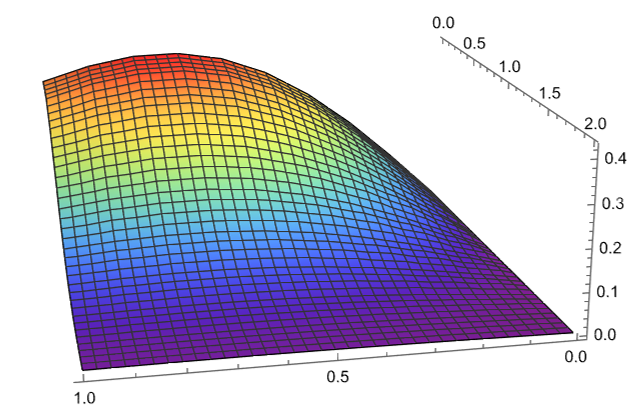
\includegraphics[width=0.5\textwidth]{ser_graph}%
	\caption{Кручение стержня прямоугольного сечения}
	\vspace*{-2mm}
	\label{pic1}
\end{figure}
\begin{figure}[!h]
	\centering
	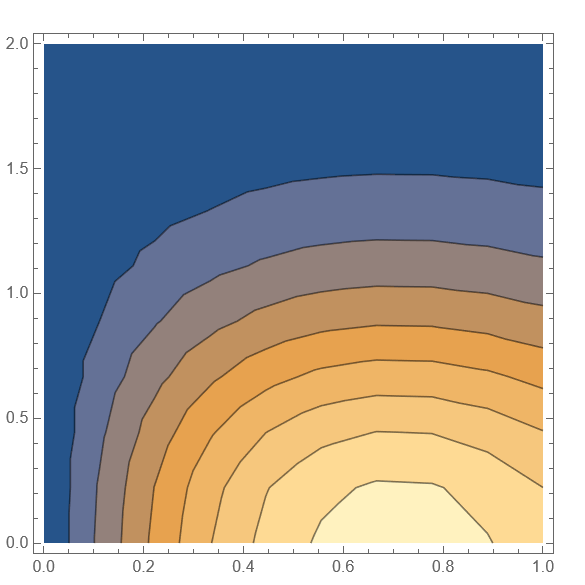
\includegraphics[width=0.5\textwidth]{ser_levels}%
	\caption{Кручение стержня прямоугольного сечения}
	\vspace*{-2mm}
	\label{pic1}
\end{figure}

\section{Решение задачи о кручении стержня методом Ритца}
Решение задачи кручения стержня прямоугольного сечения~\cite{Michilin}, как уже было показано выше,  сводится к интегрированию уравнения Пуассона~(\ref{funCruc})
 \[
-\Delta \psi = 2G \theta,
\]
где $G$~--- модуль сдвига, $\theta$~--- угол закручивания стержня на единицу
его длины, в прямоугольнике
\[
-a \leqslant x \leqslant a, -b \leqslant y \leqslant b
\]
при краевых условиях
\[
\psi(\pm a, y) =  \psi(x,\pm b) = 0.
\]

Полагая для упрощения $\psi = 2G \theta u$, получим задачу в виде
\begin{equation}
	\label{phi_ Poisson_2}
	\begin{cases}
	-\Delta u = 1, \\
	u(\pm a, y) =  u(x,\pm b) = 0.
	\end{cases}
\end{equation}

Применим метод Ритца, взяв за координатные функции полиномы.
Из соображений симметрии ясно, что функция $u(x, y)$ четна
как по~$x$, так и относительно~$y$. Такие многочлены, равные нулю на контуре прямоугольника, т.\,е. на прямых $x = \pm a$, $y = \pm b$ имеют вид
\begin{equation}\label{poly_Ritz}
	(x^2 - a^2)(y^2 - b^2)(a_1 + a_2x^2 + a_3 y^2 + \ldots)
\end{equation}

Ограничимся тремя членами и положим приближенно
\begin{equation}\label{u_3_poly_Ritz}
	u \approx u_3 = (x^2 - a^2)(y^2 - b^2)(a_1 + a_2 x^2 + a_3 y^2).
\end{equation}

Найдя соответствующие производные и приравняв их нулю, получим систему линейных алгебраических уравнений  Ритца, вида~\eqref{Ritz_F_system}, решение которой
в данном случае
\begin{equation}\label{a_123_Ritz}
	\begin{cases}
	a_1 = \frac{35 (9a^4 + 130 a^2 b^2 + 9 b^4)}
	{16 (45 a^6 + 509 a^4 b^2 + 509 a^2 b^4 + 45 b^6)},\\
	a_2 = \frac{105 (9a^2 + b^2)}
	{16 (45 a^6 + 509 a^4 b^2 + 509 a^2 b^4 + 45 b^6)},\\
	a_3 = \frac{105 (a^2 + 9 b^2)}
	{16 (45 a^6 + 509 a^4 b^2 + 509 a^2 b^4 + 45 b^6)}.\\
	\end{cases}
\end{equation}
Рассмотрим график и линии уровни функции~\eqref{u_3_poly_Ritz}
\begin{figure}[!h]
	\centering
	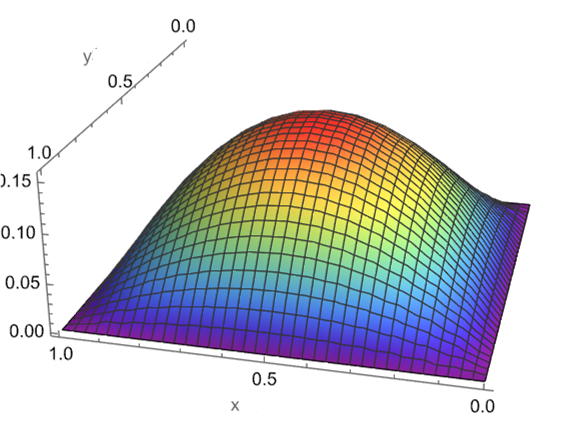
\includegraphics[width=0.5\textwidth]{ritz_graph}%
	\caption{Кручение стержня прямоугольного сечения}
	\vspace*{-2mm}
	\label{pic1}
\end{figure}
\begin{figure}[!h]
	\centering
	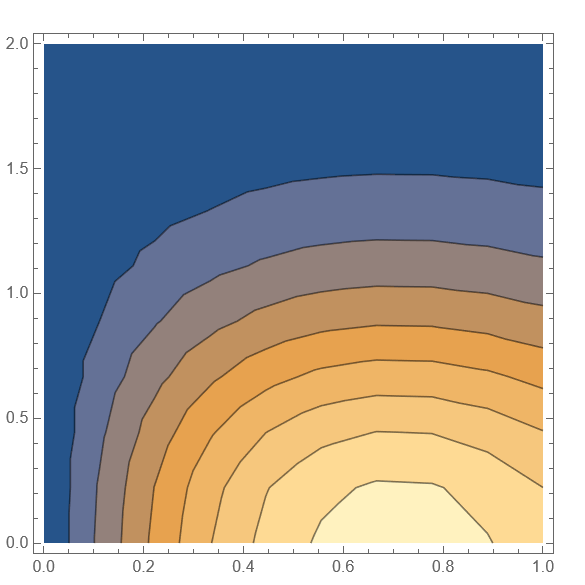
\includegraphics[width=0.5\textwidth]{ritz_levels}%
	\caption{Кручение стержня прямоугольного сечения}
	\vspace*{-2mm}
	\label{pic1}
\end{figure}

\newpage
\section-{Заключение}
В ходе выполнения курсовой были изучены методы интегрирования и обобщенных функций нахождения уравнения упругого изгиба стержня.	
С помощью этих методов были решены два типа задач, их результаты оказались идентичны.
Метод интегрирования является более трудоемким и менее удобным по сравнению с методом обобщенных функций, так как требует учета большего количества граничных условий и большего объема вычислений.
\newpage
\begin{thebibliography}{2}
\bibitem{Michilin} С. Г. Михлин. Вариационные методы в математической физике, М.: Изд-во Наука, 1970. --- 512~с.

\bibitem{Temochenko75} С. П. Тимошенко, Дж. Гудьер. Теория упругости, М.: Изд-во Наука, 1975. --- 576~с.

\bibitem{MICHLIN_SMOLICKY} 
	
\end{thebibliography}

\end{document} 